\documentclass[oneside,a4paper,12pt]{article}
\usepackage{graphicx}
\usepackage{amsmath}
\usepackage{listings}
\graphicspath{{~/templates/}, {../images/}}

\makeindex
\begin{document}
	\begin{titlepage}
		\includegraphics[width=4cm]{logopopo.png}
		\hspace*{\fill}
		\includegraphics[width=6cm]{logouniv.png}
		
		\begin{center}
			\vspace{1cm}
			\textbf{TP Support de Transmission}\\
			\textbf{Amplificateur Equilibré}\\
			\vspace{1cm}
			\textbf{Maxence LAURENT, Thibault VOLLERIN, Maxence NEUS}\\
			\vspace{3cm}
			%\includegraphics[width=13cm]{titlepage.png}\\
			\vspace{\fill}
			\textbf{Mars 2022}\\
		\end{center}
	\end{titlepage}
	
	\tableofcontents
	
	\vspace{5cm}
	
	%\section{Introduction}
	\begin{abstract}
	Le but de ce TP est de comprendre le fonctionnement des coupleurs hybrides. Dans un premier temps, 
	nous devons étudier un coupleur seul afin de déterminer sa matrice S et d’en déduire le rôle des différentes sorties. 
	Dans un second temps, nous devons analyser un amplificateur et pour finir créer un amplificateur équilibré en assemblant les coupleurs aux amplificateurs. 
	Tout cela est réalisé à l’aide un VNA (Vectorial Network Analyser).
 	\end{abstract}

	\newpage

	\section{Préparation}
	\subsection{Caractèrisation des composants seuls}
	Un coupleur parfait à une Isolation = 0, pas de pertes et un coefficient de réflexion nul.
	Les coupleurs hybrides possèdent un déphasage entre la voie couplée et la voie directe et 
	la puissance incidente se répartit de manière identique sur la voie couplée et la voie directe.\\
	On donne la matrice [S] d'un tel coupleur.

	\begin{figure}[h]
		\center
		$
		\begin{pmatrix}
		0 & \beta & 0 & \delta \\
		\beta & 0 & \delta & 0 \\
		0 & \delta & 0 & \beta \\
		\delta & 0 & \beta & 0
		\end{pmatrix}
		$
	\caption{Martice [S] du coupleur parfait}
	\end{figure}
	
	avec 
	\[\beta = \frac{1}{\sqrt 2}e^{j \theta} \]
	\[\delta = \frac{1}{\sqrt 2}e^{j \theta + 90 ^{o} } \]

	On peut donner également la matrice S de l'amplificateur

	\begin{figure}[h]
		\centering
		$
		\begin{pmatrix}
		\rho & 0 \\
		A & S_{22} \\
		\end{pmatrix}
		$
	\caption{Martice [S] de l'amplificateur}
	\end{figure}
	\newpage
	\subsection{Coefficient de réflexion à l'entrée}
	\[ \Gamma_{e} = \frac{|b_{1}|}{|a_{1}|} \] 
	avec à l'entrée 1 du premier coupleur : $ |b_{1}| = \beta |a_{2}| + \delta |a_{4}| $ \\
	On defini $ (a^{A};b^{A}) $ $ (a^{B};b^{B}) $  les puissances à l'entrée et à la sortie 
	respectivement de l'amplificateur A et de l'amplificateur B. \\
	On a alors les relations suivantes: \\
	\[ a_{2} = b^{A}_{1} = \rho a^{A}_{1}; a_{4} = b^{B}_{1} = \rho a^{B}_{1}\]
	donc 
	\[ |b_{1}| = \beta \rho |a^{A}_{1}| + \delta \rho |a^{B}_{1}| \]
	par ailleurs 
	\[ |a^{A}_{1}| = |b_{2}| = \beta |a_{1}|; |a^{B}_{1}| = |b_{4}| = \delta |a_{1}| \]
	donc 
	\[ |b_{1}| = |a_{1}|(\beta^{2} \rho + \delta^{2} \rho) \]

	d'o\`u
	\[ \Gamma_{e} = \frac{|b_{1}|}{|a_{1}|} = \rho(\beta^{2} + \delta^{2}) \]

	\subsection{Gain en puissance}

	D'après la matrice [S] du coupleur, on a en voie couplée $ b_{4} = \delta a_{1} + \beta a_{3} $
	et en voie directe $ b_{2} = \beta a_{1} + \delta a_{3} $ avec $ a_{1} = P_{INC} $ et $ a_{3} = 0 $ en voie isolée.
	
	De plus en sortie des deux amplificateurs $ b_{2} = A a_{1} $.

	En combinant ces deux équations, on obtient:
	\[ b_{2} = \delta A \beta a_{1} + \beta A \delta a_{1} \]
	d'o\`u 
	\[ b_{2} = (2 \delta A \beta) a_{1} \]
	
	Soit un gain global de $ 2 \delta A \beta $.
	\newpage

	\section{Manipulations}
	\subsection{Calibrage}
	Afin de pouvoir utiliser le VNA, nous devions d’abord le calibrer.\\ 
	Pour cela nous avons fait un calibrage de type SOLT (Short Open Load Thru).\\
	Ce calibrage utilise 3 types d’étalons (short, open et load) qui sont fournis par le fabricant.

	Avant le calibrage, il faut:
	\begin{itemize}
		\item Régler la puissance (-10 dBm) car le VNA sature à 27 dBm. Cependant, les amplificateurs ont un gain de 15 dB et le VNA à des difficultés au dessus de quelques dBm.
		\item Régler la gamme de fréquence entre 100MHz et 5GHz.
		\item Le nombre de points à 401.
	\end{itemize}

	Une fois les paramètres appliqués, nous avons utilisé un kit de calibrage de type CAL/CAL KIT afin d’opérer le calibrage SOLT.

	Une fois le calibrage effectué, nous avons vérifié que nous avions les bonnes valeurs pour S11 et S22.

	Nous avons obtenu $S_{11} = -\infty$, $S_{12} = 0 dBm$, $S_{21} = 0 dBm$, $S_{22} = -\infty$, ce qui montre le bon calibrage du VNA. 

	\begin{figure}[h]
		\centering
		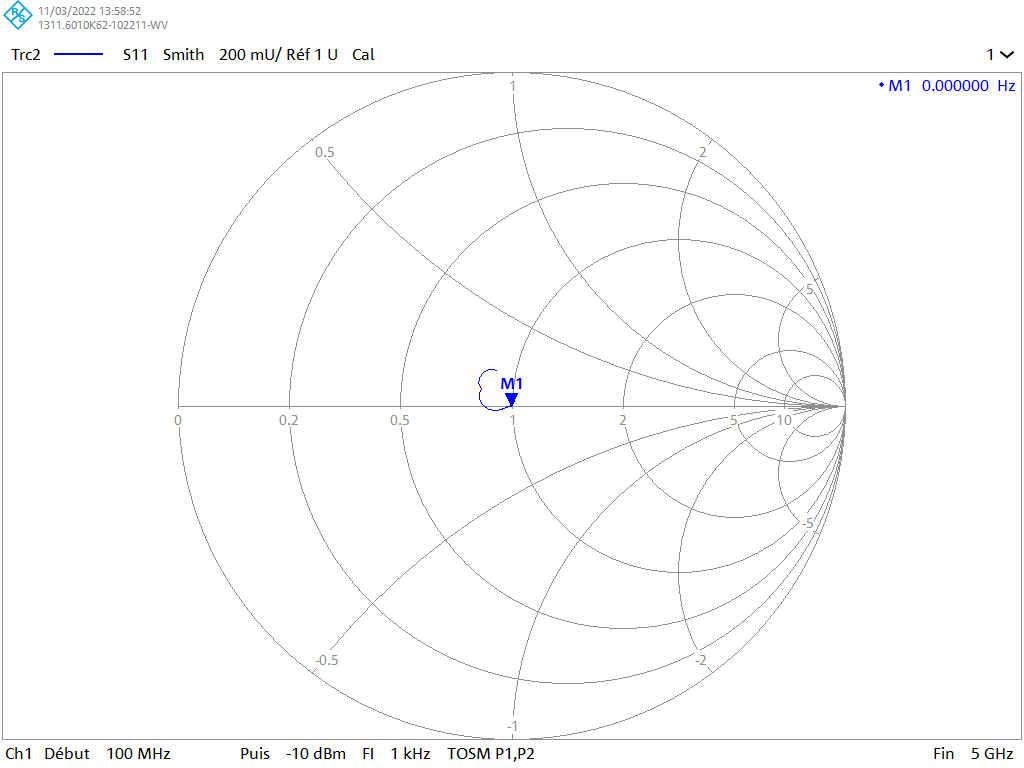
\includegraphics[width=9.5cm]{calibrage.png}
		\caption{Calibrage du VNA}
	\end{figure}

	\subsection{Mesure de la matrice [S] du coupleur}
	Notre coupleur possédait 4 pôles, ce qui nous fait 16 coefficients. 
	Cependant, nous avions besoin de déterminer seulement 4 coefficients pour connaître sa matrice S (symétrie du coupleur). 
	Ces 4 coefficients ont été déterminés sur une bande allant de 100 MHz à 5 GHz. 
	Nous avons pris une fréquence au centre de cette bande (2,45 GHz).

	\paragraph{a.}\paragraph{}
	\begin{figure}[h]
		\centering
		$
		\begin{pmatrix}
			-32 dB & -31 e^{j(-178.5^{o})} dB & -2.8 e^{j(-118^{o})} dB & -3.3 e^{j(155.6^{o})} dB \\
			-31 e^{j(-178.5^{o})} dB & -22 dB & -3.3 e^{j(155.6^{o})} dB & -2.8 e^{j(-118^{o})} dB \\
			-2.8 e^{j(-118^{o})} dB & -3.3 e^{j(155.6^{o})} dB & -20.7 dB & -31 e^{j(-178.5^{o})} dB \\
			-3.3 e^{j(155.6^{o})} dB & -2.8 e^{j(-118^{o})} dB & -31 e^{j(-178.5^{o})} dB & -41.5 dB \\
		\end{pmatrix}
		$
		\caption{Matrice [S] experimentale du coupleur seul}
	\end{figure}

	\paragraph{b.}
	Une fois que nous avons déterminé ces 4 paramètres, nous pouvons déduire que:

	\begin{itemize}
		\item[Couplage] = -3 dB
		\item[Isolation] = -31 dB 
		\item[Coefficient de réflexion] = -32 dB
		\item[Pertes d'insertion] = -3.3 dB  
		\item[Bande Passante à 1dB] : entre 800MHz et 4.2GHz 
	\end{itemize}
	
	\paragraph{Calcul des pertes Joules}
	\paragraph{}
	On a en linéaire l'équation suivante : 
	\[ 1 = \frac{P_{r}}{P_{1}} + \frac{P_{2}}{P_{1}} + \frac{P_{3}}{P_{1}} + \frac{P_{4}}{P_{1}} + \frac{P_{J}}{P_{1}} + \]

	On en déduit $ P_{J} $:
	\[ P_{J} =  \]

	\paragraph{c.}
	\begin{figure}
		\centering
		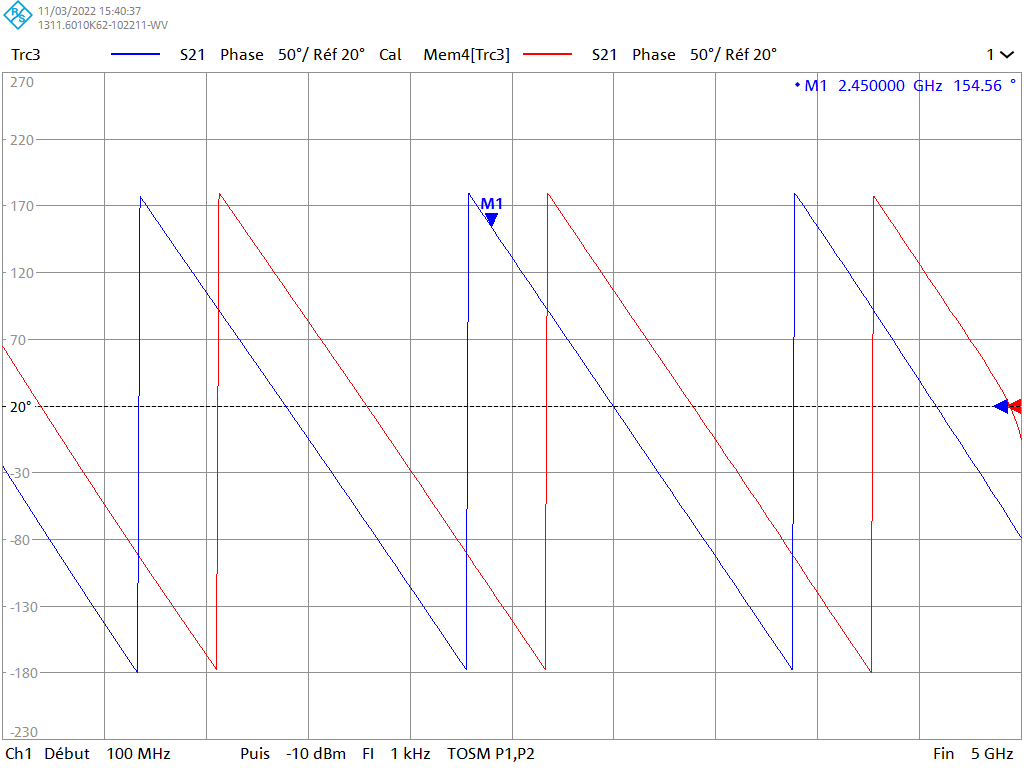
\includegraphics[width=10cm]{S14(bleu)-S13(rouge).png}
		\caption{Phases de $S_{14}$ (en bleu) et $S_{13}$ (en vert)}
	\end{figure}

	On observe ici les phases de $S_{1i}$ pour les deux sorties qui sont les sorties couplée et directe.
	On observe une différence constante de phase de 90° entre ces deux sorties. On en déduit que notre coupleur est un coupleur hybride 90°. 

	La position de ces deux courbes de phases nous indique que la sortie 3 est la sortie couplée et la 4 la sortie directe.

	\paragraph{d.}
	\paragraph{}
	\begin{figure}[h]
		\centering
		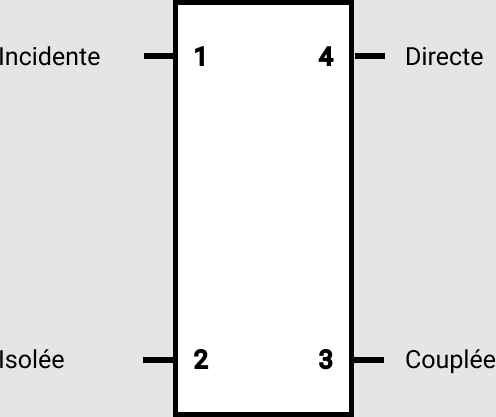
\includegraphics[width=6.5cm]{Coupleur.png}
		\caption{Schéma du coupleur}		
	\end{figure}

	\subsection{Mesure de la matrice [S] des amplificateurs}
	\paragraph{Amplificateur seul} \paragraph{}
	On a mesuré les coefficients de la matrice [S] d'un amplificateur:
	\begin{figure}[h]
		\centering
		$
		\begin{pmatrix}
			-16.8 dB & 16 dB \\
			-22 dB & -22 dB \\
		\end{pmatrix}
		$
		\caption{Matrice [S] de l'amplificateur}
	\end{figure}

	On extrait les Caractèristiques de l'amplificateur:
	\begin{itemize}
		\item[Gain] = 16dB
		\item[Coefficient de réflexion] entrée: -16dB ($S_{11}$)
		\item[Coefficient de réflexion] sortie: -22dB ($S_{22}$)
		\item[Isolation] = -22 dB ($S_{12}$)  
	\end{itemize}

	\paragraph{Amplificateur equilibré} \paragraph{}

	On a également mesuré les coefficients de la matrice [S] du montage complet
	
	\begin{figure}[h]
		\centering
		$
		\begin{pmatrix}
			-26.8 dB & 15.6 dB \\
			-23 dB & -22 dB \\
		\end{pmatrix}
		$
		\caption{Matrice [S] de l'amplificateur equilibré}
	\end{figure}

	\newpage
	\begin{figure}[h]
		\centering
		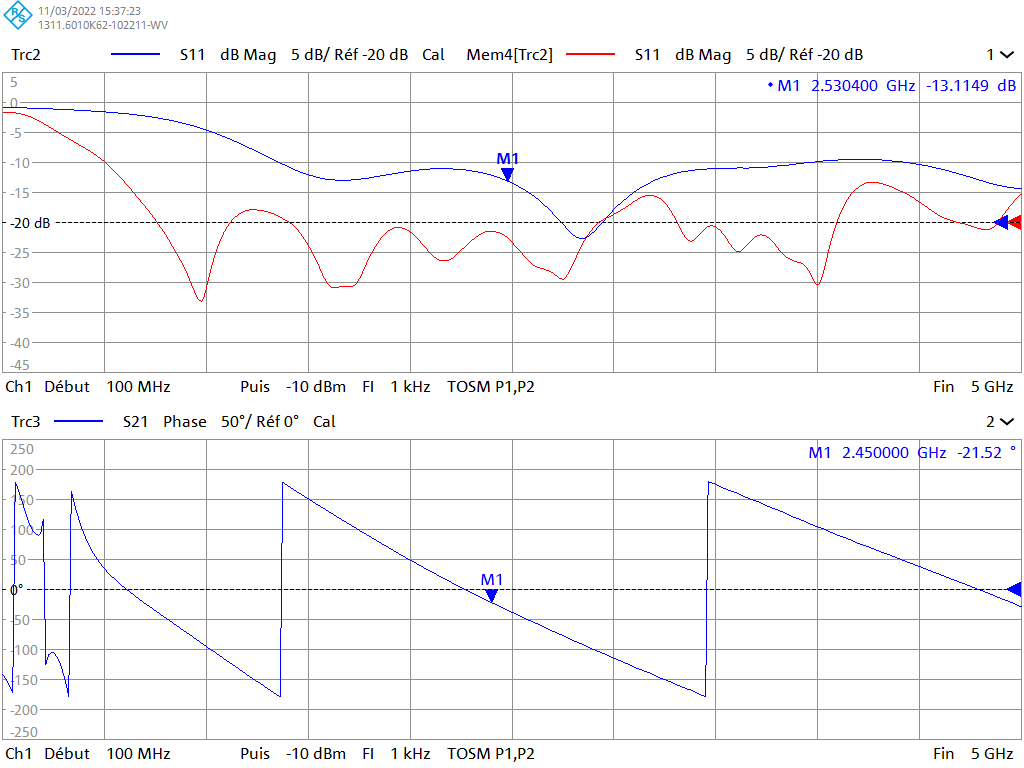
\includegraphics[width=10cm]{S11AMpliComparaison.png}
		\caption{Comparaison des coefficients de réflexion des deux montages}
	\end{figure}

	On observe que le montage amplificateur equilibré a un coefficient de réflexion bien moindre sur la globalité de la bande mesurée.

	\newpage
	\section{Conclusion}
	Ce TP nous a permis de mieux comprendre le fonctionnement des coupleurs hybrides et de prendre en main le VNA. 
	Tout d’abord, nous avons pu étudier un coupleur seul et déterminer sa matrice S. 
	Nous avons donc pu comprendre son fonctionnement, trouver ses paramètres et ainsi déduire ses différentes voies afin de l’assembler avec un amplificateur. 
	Ensuite, nous avons étudié deux amplificateurs pour déterminer leur coefficient de réflexion et leur gain. 
	Pour finir, nous avons représenté le montage d’un amplificateur équilibré. 
	Nous avons pu voir l’intérêt des coupleurs qui permettent d’atténuer la puissance 
	d’entrée pour éviter la saturation de l’amplificateur (Premier coupleur) et en sortie d’annuler cette atténuation une fois le gain de l’amplificateur appliqué (Deuxième coupleur).
	
	\newpage
	\appendix
	\section{Annexe}

	\begin{figure}[h]
		\centering
		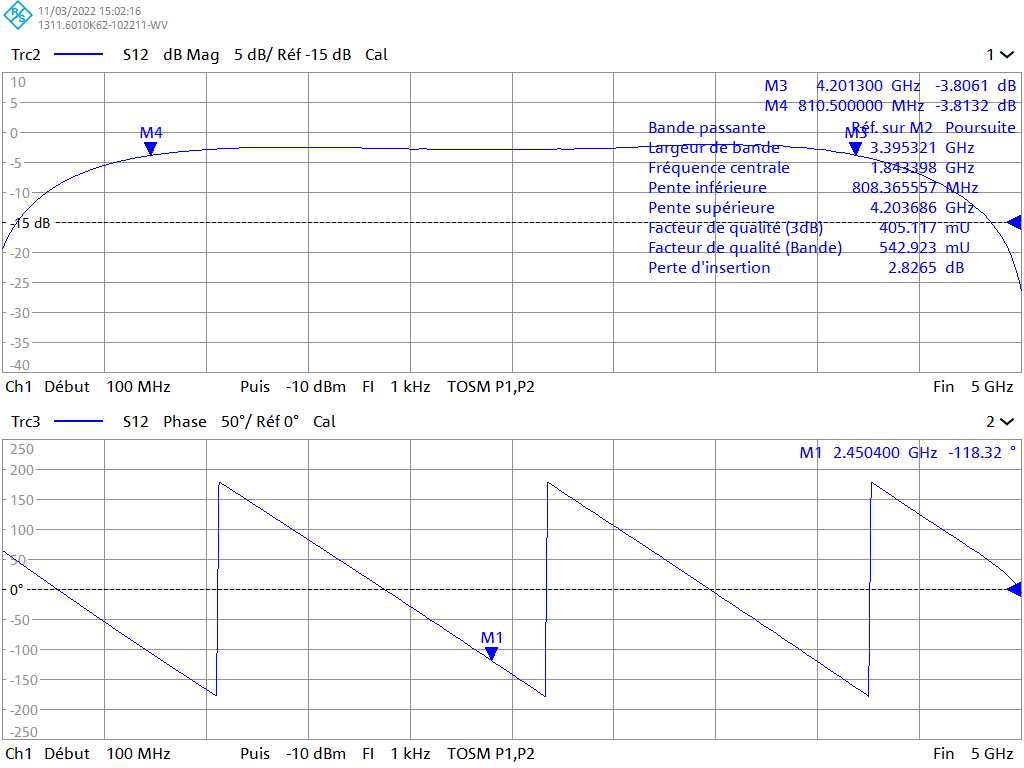
\includegraphics[width=10cm]{BandePassante1dB.png}
		\caption{Bande passante à 1dB de l'amplificateur seul}
	\end{figure}

\end{document}
